\section{Implementation}
\label{sec:compile}

The implementation for my semester project is hosted on \href{https://github.com/bennn/rkt-kodkod}{Github}.
Currently the implementation is 2,500 lines of Racket code and implements a compiler from \emph{propositional} logic to CNF.

\begin{figure}[t]
  \label{fig:lang}
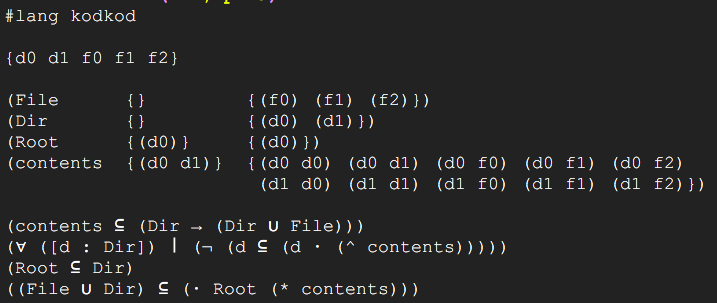
\includegraphics[width=10cm]{rkt.png}

  \vspace{0.1cm}
  %\hrule
  \hrule\hrule
  %\vspace{0.1cm}

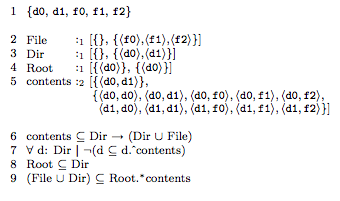
\includegraphics[width=10cm]{fs.png}
\caption{Racket code vs. mathematical specification}
\end{figure}

The surface syntax (\figref{fig:lang}) directly follows the formal syntax of relational logic.
Logic problems are written naturally with sets for atoms \& bounds and
 unicode for logical operators.
Typographical errors in the problem spec are reported in terms of source code
 lines and positions.

After reading a file into a data structure representing a relational logic
 formula, we compile the formula to a boolean matrix representation.
Like Kodkod, this matrix is implemented sparsely.
We do not, however, have a skolemizer or symmetry detector.
Instead matrices are compiled na\"ively, with only the most obvious short-circuit
 optimizations.

Once the problem is translated to a matrix, we compile a boolean circuit and
 then translate the circuit to CNF.
The circuits do as much collapsing as is possible; for many formulas
 we can output SAT or UNSAT at this stage without calling an external solver,
 so this is where the project ends for the moment.


\subsection{Challenges}

The most difficult part of the project was choosing what to implement to
 reach deliverable checkpoints.
I did poorly at this task.
Reading the dissertation was informative, but focused primarily on Kodkod's
 technical contributions rather than on the details needed to walk a complete
 path from specification to SAT/UNSAT.
For example, I initially misunderstood that the boolean matrix representation
 is only for expressions and relational bounds, but \emph{not} for top-level
 formulas and constraints.
It was only after implementing most of an interpreter that I realized the dead-end.

Unfortunately the Java code was even worse to read due to a very high signal-to-noise
 ratio.
Kodkod is full of factories and generic class hierarchies that tend to obsure
 the purpose of each component, at least to someone unaccustomed to reading
 Java code.\footnote{Maybe my biggest problem was refusing to use an IDE like Eclipse or IntelliJ.}
There were also many diversions in the name of ease and optimization\textemdash
 rather than puzzle over the big picture of the code, it was easier to latch
 on to a data structure like the sparse-sequence-backed matrices and their
 supporting red-black tree data structure.
Implementing these was fun and interesting to think about how best to translate
 from Java, but ultimately did little to advance my goal of porting the Kodkod solver.


\subsection{Comparisons}

Some benefits of the rewrite over the original:
\begin{itemize}
\item The mathematical front-end syntax is much easier to use (and program)
 than Kodkod's Java API.
\item Racket's pattern-matching and variable-arity functions
 are concise alternatives to visitor and factory patterns.
\item Stateful, object-based data structures are almost all replaced with
 functional versions.
 Though, I have not benchmarked to see if this gave a performance improvement.
\end{itemize}

